\begin{ledgroupsized}[r]{120mm}
\footnotesize
\pstart
\noindent\textbf{Überlieferung:}
\pend
\end{ledgroupsized}
\begin{ledgroupsized}[r]{114mm}
\footnotesize
\pstart
\parindent -6mm
\makebox[6mm][l]{\textit{L}}%
Konzept:
LH~XXXV~9, 10~Bl.~1\textendash2. 
Ein Bogen~2\textsuperscript{o};
\href{\Scan{LH_35_09_10_001wz}}%
{Wasserzeichen} in Bl.~1.
Dreieinhalb %
Seiten;
untere Hälfte von Bl.~2~r\textsuperscript{o} leer.
Bei der Anfertigung der Zeichnungen \lbrack\textit{Fig.~3}\rbrack\  und \lbrack\textit{Fig.~4}\rbrack\ auf
Bl.~\href{\Scan{LH_35_09_10_001v}}{\lbrack1~v\textsuperscript{o}\rbrack}
hat Leibniz sich an den mit Zirkel gestochenen Punkten und den durch das Blatt durchscheinenden Konturen der Diagramme \lbrack\textit{Fig.~1}\rbrack\  und \lbrack\textit{Fig.~2}\rbrack\ auf der Rückseite (Bl.~\href{\Scan{LH_35_09_10_001r}}{1~r\textsuperscript{o}}) orientiert.
\pend
\end{ledgroupsized}
\selectlanguage{french}
\vspace{8mm}
\pstart
\centering
\edlabel{35_09_10_001-002_1a}%
\edtext{}{\xxref{35_09_10_001-002_1a}{35_09_10_001-002_1b}%
\lemma{\href{\Scan{LH_35_09_10_001r}}%
{\lbrack1~r\textsuperscript{o}\rbrack}}\Bfootnote{%
\textit{(1)}~Invention et demo %
\textit{(2)}~Demonstration analytique du principe de l'Equilibre 
\bars{, \bars{c'est à dire \textit{erg.}} 
qui fait voir en même temps l'origine 
\textit{(1)}~de l'invention
\textit{(2)}~de son invention~\textit{gestr.}} 
\lbrack/\rbrack\
\bars{Soyent les \textit{erg.}} corps~\textit{L}}}%
\href{\Scan{LH_35_09_10_001r}}%
{\lbrack1~r\textsuperscript{o}\rbrack}
\hfill
Demonstration analytique du principe\indexS{principe de l'Equilibre} de l'Equilibre\indexS{demonstration du principe de l'Equilibre}\indexS{demonstration analytique du Principe de l'Equilibre}
\hfill
\phantom{\lbrack1~r\textsuperscript{o}\rbrack}
\pend
\nobreak
\vspace{0.5\baselineskip}
\pstart
\noindent 
\edlabel{35_09_10_001-002_9a}%
\edtext{}{%
\xxref{35_09_10_001-002_9a}{35_09_10_001-002_9b}%
\lemma{Soyent \bracks{...} par \textit{DF}}%
\Cfootnote{%
Leibniz hat an dieser Stelle eine Passage aus dem Zeugen \textit{L\textsuperscript{1}} von N.\;\ref{57033+41135} abgeschrieben, die er dort nachträglich eingefügt und in \textit{L\textsuperscript{2}} nicht übernommen hatte: \refpassage{37_03_064_3a}{37_03_064_3b}.}}%
Soyent les corps\edlabel{35_09_10_001-002_1b}
donnés representés par les droites (ou cylindres egalement epais 
dont la longueur quelconque est en raison des corps) \textit{DEF}, \textit{ACB},
\edtext{attachées par}{%
\lemma{attachées}%
\Bfootnote{%
\textit{(1)}~à
\textit{(2)}~par~\textit{L}}}
leur points de milieu à la balance\indexS{corps suspendus d'une balance} \textit{CGE} soûtenue 
\edtext{par \textit{PGQ}}{\lemma{par}\Bfootnote{%
\textit{(1)}~l'axe %
\textit{(2)}~\textit{PGQ}~\textit{L}}}
axe\indexS{axe} perpendiculaire à \textit{CGE} tellement pris, et \textit{ACB} tellement inclinée, qu'en supposant \textit{BXZ} (partie de \textit{ACB}) egale à \textit{DEF} 
\edtext{soient \textit{EG}, \textit{XY}}{\lemma{soient}\Bfootnote{%
\textit{(1)}~leur points de milieu %
\textit{(2)}~les di %
\textit{(3)}~\textit{XY}, \textit{E} %
\textit{(4)}~\textit{EG}, \textit{XY}~\textit{L}}}
distances de leur points de milieu \textit{E}, \textit{X}, de l'axe \textit{PGYQ} égales; 
\edtext{et que \textit{ARZ} (reste de \textit{ACB}) soit}{\lemma{et}\Bfootnote{%
\textit{(1)}~le reste 
\textit{(2)}~\textit{AZ} %
\textit{(3)}~que \textit{ARZ} (reste de \textit{ACB}) soit~\textit{L}}}
coupé en 
\edtext{deux egalement}{\lemma{deux}\Bfootnote{%
\textit{(1)}~par %
\textit{(2)}~egalement~\textit{L}}}
au point de 
\edtext{milieu\indexS{point de milieu} \textit{R}, par}{\lemma{milieu \textit{R},}\Bfootnote{%
\textit{(1)}~par l'axe \textit{PRG} %
\textit{(2)}~par~\textit{L}}}
le dit axe\indexS{axe} \textit{PRG}. Il s'agit de trouver le point \textit{G} ou axe \textit{PG}; 
et l'inclination de \textit{ACB} ou l'angle \textit{ACE} tel qu'il faut pour cet 
\edlabel{35_09_10_001-002_2a}%
\edtext{}{\xxref{35_09_10_001-002_2a}{35_09_10_001-002_2b}\lemma{effect.}\Bfootnote{%
\textit{(1)}~Cela estant une %
\textit{(2)}~Cecy %
\textit{(3)}~Cela est un problemen purement
\textit{(4)}~Ce probleme est donc~\textit{L}}}%
effect.
\pend
\begin{edfigure}%
\hfill
\includegraphics[scale=1]{%
gesamttex/edit_VIII-4/images/LH_35_09_10_001-002_d1_001r.pdf}
\hspace*{10mm}%
\includegraphics[scale=1]{%
gesamttex/edit_VIII-4/images/LH_35_09_10_001-002_d2_001r.pdf}
\hfill
\edcaption{\pagelabel{Fig:35_09_10_001-002_fig-1}%
\lbrack\textit{Fig.~1, tlw. Blindzeichnung}\rbrack 
\hspace*{26mm}%
\lbrack\textit{Fig.~2, tlw. Blindzeichnung}\rbrack\hspace*{12mm}}
\end{edfigure}
\pstart 
Ce probleme est donc\edlabel{35_09_10_001-002_2b} 
purement Geometrique au quel nous avons reduit ce grand Probleme de\indexS{grand probleme de mecanique} 
\edtext{Mechanique: et}{\lemma{Mechanique:}\Bfootnote{%
\textit{(1)}~Car %
\textit{(2)}~et~\textit{L}}}
il est manifeste que \textit{G} sera le point 
\edtext{d'equilibre\indexS{point d'equilibre}\indexS{equilibre} demandé. Car \textit{ARZ}. est en}{\lemma{d'equilibre}\Bfootnote{%
\textit{(1)}~, parce que %
\textit{(2)}~demandé. %
\textit{(a)}~Puisque %
\textit{(b)}~Car \textit{ARZ}. est \bars{manifestement \textit{gestr.}} en~\textit{L}}}
equilibre par luy même (puisque il est coupé au milieu 
\edtext{\textit{R}}{\lemma{}\Bfootnote{\textit{R} \textit{erg.~L}}} 
par l'axe\indexS{axe} \textit{PRG}.) et \textit{ZB} est contrabalancée par \textit{DF}%
\edlabel{35_09_10_001-002_9b}
(puisqu'elles sont egales et ont leurs points de milieu\indexS{point de milieu} egalement distans
de l'axe.) donc tout est en equilibre\indexS{equilibre} à l'egard de 
\edtext{l'axe \textit{PGQ}.}{\lemma{l'axe}\Bfootnote{%
\textit{(1)}~\textit{PQ} %
\textit{(2)}~\textit{PGQ}.~\textit{L}}} 
\pend
\pstart 
Pour trouver le point \textit{G} considerons que les triangles \textit{RGC}, \textit{RYX} sont semblables donc \textit{GC} à \textit{YX}, c'est à dire \textls{\textit{GC} à} 
\edtext{\lbrack\textls{\textit{EG}}\rbrack}{\lemma{}\Bfootnote{\textls{\textit{CG}} \textit{L ändert Hrsg.}}}
\textls{comme \textit{RC} à \textit{RX}}. Or \textit{RC} est $AC-AR$ et \textit{AR} moitié de \textit{AZ} 
(et \textit{AZ} est $AB-ZB$ ou $AB-DF$. donc
\edtext{la moitié de \textit{AZ}, ou}{%
\lemma{la moitié de \textit{AZ},}%
\Bfootnote{%
\textit{(1)}~est
\textit{(2)}~ou~\textit{L}}}
\textit{AR}) est $AC-DE$. 
Donc \textit{RC} est $AC-AC+DE$. C'est à dire
\edtext{\textls{\textit{RC} est égale à \textit{DE}} ou \textit{XB} ou \textit{XZ}. De plus puisque}{%
\applabel{FnB:35_09_10_001-002_est-egale}%
\lemma{\textls{\textit{RC} est}}\Bfootnote{%
\textit{(1)}~\textls{\textit{DE}}
\textit{(2)}~\textls{égale à \textit{DE}}
\bars{\textit{(1)}~ou \textit{XR} ou \textit{X} %
\textit{(2)}~ou \textit{XB} ou \textit{XZ}. \textit{erg.}}
\textit{(a)}~De même \textit{RX} est égal %
\textit{(b)}~De %
\textit{(c)}~Donc \textit{RX} ou \textit{RC} égale à \textit{XB}. Donc \textit{RX} egale \textit{CB} ou \textit{AC}. Et de \textit{RX} et \textit{AC} egales ostant \textit{ZX} et \textit{RC} egales resteront %
\textit{(d)}~Or puisque %
\textit{(e)}~De plus puisque~\textit{L}}}
\textit{AR} doit estre egale 
\edtext{à \textit{RZ}, à}{%
\lemma{à \textit{RZ},}%
\Bfootnote{%
\textit{(1)}~à choses egales %
\textit{(2)}~à~\textit{L}}}
ces droites egales adjoutons autres droites egales, \textit{RC}, \textit{ZX}, les sommes \textls{\textit{AC}, \textit{RX} seront} 
\edtext{\textls{égales}. \edlabel{35_09_10_001-002_10a}%
Donc \textls{\textit{GC} à} \lbrack\textls{\textit{EG}}\rbrack\ estant}{\lemma{\textls{égales}.}\Bfootnote{%
\textit{(1)}~Donc %
\textit{(2)}~Donc \textls{\textit{GC}} %
\textit{(a)}~\textls{sera} %
\textit{(b)}~\textls{estant à \textit{CG}} %
\textit{(c)}~\textls{à} 
\bars{\textls{\textit{CG}} \textit{ändert Hrsg.}} 
estant~\textit{L}}}
comme \textit{RC} à \textit{RX} sera comme \textit{DE} à \textit{AC}, c'est à dire \textls{comme \textit{DF} à \textit{AB}}. Et le point \textit{G} coupant la droite donnée, \textit{CE} en raison donnée \textit{DF} à \textit{AB} (c'est à dire en raison reciproque des poids\indexS{raison reciproque de deux poids}) sera trouvé. Ce qu'il falloit faire.%
\edlabel{35_09_10_001-002_10b}
\pend
\pstart
Le point \textit{G} estant trouvé il est aisé, mais il n'est pas necessaire de 
\edlabel{35_09_10_001-002_6a}%
\edtext{}{%
\xxref{35_09_10_001-002_6a}{35_09_10_001-002_6b}%
\lemma{trouver}\Bfootnote{%
\textit{(1)}~l'inclination de %
\textit{(2)}~l'angle %
\textit{(a)}~\textit{ABC} %
\textit{(b)}~\textit{ACE} %
\textit{(aa)}~propre à cette demonstration. Car prenant \textit{GV} égale à %
\textit{(bb)}~.~Neantmoins pour ne rien laisser en arriere, prenons
\textit{(cc)}~.~Car \bars{il est manifeste que \textit{erg.}} toute \bracks{...} l'equilibre %
\textit{(aaa)}~pourveu que l'on tourn %
\textit{(bbb)}~, quand \lbrack...\rbrack\ de part et %
\textit{(aaaa)}~de %
\textit{(bbbb)}~d'autre, %
\textit{(aaaaa)}~il s'approche %
\textit{(bbbbb)}~ce qui s'approché de l'axe \textit{PQ} est tousjours egal semblable et semblablement située
\textit{(ccccc)}~il \lbrack...\rbrack\  éloigne. Et %
\textit{(aaaaa-a)}~nostre %
\textit{(bbbbb-b)}~\textls{la demonstration} %
\textit{(aaaaa-aa)}~du centre %
\textit{(bbbbb-bb)}~\textls{de l'equilibre} \lbrack...\rbrack\ \textls{autres}. Neantmoins~\textit{L}}}%
trouver l'angle \textit{ACE}. Car il est manifeste que toute inclination de \textit{ACB} est indifferente à l'egard de l'equilibre,\indexS{equilibre} quand on tourne \textit{AB} sur son milieu immobile \textit{C}. 
Car tout estant égal de part et d'autre, il s'approche tousjours autant de l'axe\indexS{axe} \textit{PQ} qu'il s'en éloigne.
Et \textls{la demonstration de l'equilibre\indexS{demonstration de l'equilibre} dans une inclination de \textit{AB}, vaut pour toutes les autres}.
\pend
\pstart 
Neantmoins\edlabel{35_09_10_001-002_6b}
pour determiner l'inclination \textit{ACE} 
\edtext{si propre à monstrer}{\lemma{l'inclination}\Bfootnote{%
si \bars{si \textit{gestr.}} propre à %
\textit{(1)}~faire comprendre %
\textit{(2)}~monstrer~\textit{L}}}
le point d'equilibre,\indexS{point d'equilibre} 
\textit{G} à veue d'oeil: puisque \textit{G} est trouvé prenons \textit{GV} égale à \textit{GE}, et menons \textit{VT} parallele à 
\edtext{\textit{GQ}, et dans}{\lemma{\textit{GQ}, et}\Bfootnote{%
\textit{(1)}~tournant %
\textit{(2)}~dans~\textit{L}}}
\textit{CB} prenons \textit{BL} egale à \textit{FE} et du centre \textit{C} des points du diametre \textit{ACLB} decrivons les arcs \textit{Aa}, \textit{Bb}, \textit{LX} coupant \textit{VT} en \textit{X}, et l'inclination \textit{ARCZXb} sera telle qu'il 
\edtext{faut. Il faut}{\lemma{faut.}\Bfootnote{%
\textit{(1)}~Il est 
\textit{(a)}~nec
\textit{(b)}~seulement %
\textit{(2)}~Il faut~\textit{L}}}
seulement prendre garde, 
\edtext{que \textit{CX} ne}{\lemma{que \textit{CX}}\Bfootnote{%
\textit{(1)}~soit p %
\textit{(2)}~ne~\textit{L}}}
soit pas moindre que \textit{CV} ce qui est aisé puis qu'on n'a qu'à prendre les droites \textit{DF}, \textit{AB} assés longes, c'est à 
\edtext{dire l'épaisseur}{\lemma{dire}\Bfootnote{%
\textit{(1)}~la %
\textit{(2)}~l'épaisseur~\textit{L}}}
des cylindres assés petite. Si 
\edtext{$AB+DF$ estoit}{\lemma{$AB+DF$}\Bfootnote{%
\textit{(1)}~estoient %
\textit{(2)}~estoit~\textit{L}}}
le double de \textit{CE}\lbrack,\rbrack\ \textit{CX} seroit egale à \textit{CV} et les points 
\edtext{\textit{R}. et \textit{G}. item \textit{X}, \textit{V}, seroient}{\lemma{}\Bfootnote{%
\textit{R}. \bars{et~\textit{erg.}} \textit{G}. item \textit{X}, \textit{V}, 
\bars{et item \textit{A} et \textit{E} \textit{erg.~u.~gestr.}} seroient~\textit{L}}}
les mêmes, c'est à dire \textit{ab} 
\edtext{\textit{aRCZXb} et \textit{EC}}{\lemma{\textit{aRCZXb}}\Bfootnote{%
\textit{(1)}~sera %
\textit{(2)}~et 
\textit{(a)}~\textit{EGCV}
\textit{(b)}~\textit{EC}~\textit{L}}}
seront coincidentes. 
\edtext{Ce qui nous fournira une belle synthese que je donneray cy après.}{\lemma{Ce \lbrack...\rbrack\ après}\Cfootnote{Siehe \refpassage{35_09_10_001-002_8a}{35_09_10_001-002_8b}.}}
\pend
\selectlanguage{latin}
\vspace{0.5em} %
\pstart
\noindent
\lbrack\textit{Nachfolgend kleingedruckter Text: gestrichene Nebenrechnungen am Rand von Bl.~1~r\textsuperscript{o}}\rbrack %
\pend
\nobreak
\vspace{0.5em}
\footnotesize
\pstart
\parbox{4cm}{$AC-DE$\rule[0mm]{3mm}{0pt}$EG+CG$
\\[1ex]
\hspace*{1mm}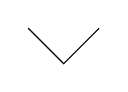
\begin{tikzpicture}\draw (0,0) -- (0.45,-0.45) -- (0.9,0); \end{tikzpicture}\hspace*{7mm}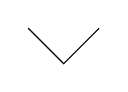
\begin{tikzpicture}\draw (0,0) -- (0.45,-0.45) -- (0.9,0); \end{tikzpicture}}
\pend
\pstart
\hspace*{3mm}\rule[-3mm]{0pt}{9mm}$\displaystyle\frac{CL}{LS} \hspace{3.5mm} \sqcap \hspace{3.5mm} \displaystyle\frac{EC}{CS}\sqcap \frac{EG}{GR}$.\quad 
$\displaystyle\frac{ER}{RS}\sqcap\frac{EG}{CG}$
\pend
\pstart
\parbox{4cm}{%
\hspace*{17mm}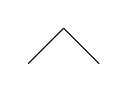
\begin{tikzpicture}\draw (0.0,-0.3) -- (-0.45,-0.75); \draw (0.0,-0.3) -- (.45,-0.75); \end{tikzpicture}
\\[-.5ex]
\hspace*{15mm}$\sqrt{LS,SE}$}
\pend
\pstart
\rule[-6mm]{0pt}{12mm}$\displaystyle\frac{ER}{RS}\sqcap\frac{EG}{CG}$.\quad
$EL^2\sqcap ME^2+CL^2$. 
\pend
\pstart
$CL^2$ 
\ledpb%
aequ. $CS^2+LS^2$
\pend
\pstart
\parbox{4cm}{%
\hspace*{12mm}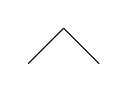
\begin{tikzpicture}\draw (0.0,-0.3) -- (-0.45,-0.75); \draw (0.0,-0.3) -- (.45,-0.75); \end{tikzpicture}
\\[-.5ex]
\hspace*{11.5mm}$LS,SE$}
\pend
\pstart
\rule[-5mm]{0pt}{10mm}%
$\displaystyle\frac{CL}{LS}\sqcap\frac{EG}{GR}$.\quad
$\displaystyle\frac{LS}{GR}\sqcap\frac{CL}{EG}$.\quad 
$\displaystyle\frac{LS}{CS}\sqcap\frac{CL}{EC}$. \qquad
$\displaystyle\frac{CL}{CS}\sqcap\frac{EG,CL}{GR,EG}$.\quad 
$\displaystyle\frac{ER}{RG}\sqcap\frac{EC}{CL}$.
\pend
\pstart
\textit{EC}. \textit{CL}. \textit{EL}. \textit{EG}. \textit{EC}. \textit{CG} datae.
\pend
\pstart
\rule[-4mm]{0pt}{11mm}%
$\displaystyle\frac{ER}{EG}\sqcap\frac{CE}{EL}$. seu $ER\sqcap\displaystyle\frac{CE,EG}{EL}$.\quad
$\displaystyle\frac{LS}{CL}\sqcap\frac{CL}{EL}$ seu $LS\sqcap\displaystyle\frac{CL^2}{EL}$
\pend
\pstart
$\displaystyle\frac{SR}{ER}\sqcap\frac{CG}{GE}$. Ergo $SR\sqcap\displaystyle\frac{ER,CG}{GE}$. 
\edtext{Ergo}{\lemma{Ergo}\Bfootnote{%
\textit{(1)}~\textit{LR} aeq. Ergo %
\textit{(2)}~$LR \;\sqcap $~\textit{L}}}
$LR \sqcap\displaystyle\frac{CL^2}{EL}+\displaystyle\frac{ER,CG}{GE}$ seu $LR \sqcap\displaystyle\frac{CL^2+CE,CG}{EL}$ et \textit{LR} ad \textit{ER}, ut $CL^2+CE,CG$ ad $CE,EG$ seu ut 
\rule[-2mm]{0pt}{9mm}%
$\displaystyle\frac{LR}{ER}\sqcap\frac{CL^2}{CE,GG}+\efrac{E}{}$ \lbrack\textit{Rechnung bricht ab.}\rbrack\
\pend
\normalsize %
\vspace{0.5em} %
\selectlanguage{french}
\pstart
\edlabel{35_09_10_001-002-analytique-a}%
\href{\Scan{LH_35_09_10_001v}}%
{\lbrack1~v\textsuperscript{o}\rbrack} 
J'appelle cette demonstration\indexS{demonstration analytique}
\edtext{analytique non pas comme si elle dependoit des symboles, car c'est une erreur ridicule de quelques uns qui s'imaginent qu'il n'y a point d'autre analyse\indexS{analyse} que l'algebre\bracks{,}\indexS{algebre} mais}{\lemma{analytique}%
\Bfootnote{%
\textit{(1)}~parce qu'elle
\textit{(2)}~\bars{%
non pas comme si elle dependoit
\textit{(1)}~de l'algebre %
\textit{(2)}~des %
\textit{(a)}~si %
\textit{(b)}~sy %
\textit{(c)}~symboles, \bracks{...} mais \textit{erg.}}
par ce~\textit{L}}} 
qu'elle monstre l'origine de l'invention,\indexS{origine de l'invention} 
car elle monstre comment on peut 
\edtext{trouver la regle}{\lemma{trouver}\Bfootnote{%
\textit{(1)}~par une voye %
\textit{(2)}~la regle~\textit{L}}}
de l'equilibre\indexS{regle de l'equilibre} par une voye asseurée, 
\edtext{sans en sçavoir rien par avance.\edlabel{35_09_10_001-002-analytique-b} Du lieu que les}{\lemma{sans}\Bfootnote{%
\textit{(1)}~la sçavoir déjà
\textit{(2)}~sçavoir déjà cette regle
\textit{(3)}~en sçavoir rien par avance. Du lieu
\textit{(a)}~que les autres demonstrations %
\textit{(aa)}~que j'ay veues n
\textit{(bb)}~que %
\textit{(cc)}~qu'on %
\textit{(aaa)}~ne %
\textit{(bbb)}~n'a p %
\textit{(b)}~que les~\textit{L}}}
demonstrations ordinaires supposent qu'on ait déjà entendu parler du
\edtext{theoreme \indexN{\textls{Archimedes} 287\textendash212 v. Chr.}d'Archimede\indexS{theoreme d'Archimede}}{\lemma{theoreme d'Archimede}\Cfootnote{Siehe \indexN{\textls{Archimedes} 287\textendash212 v. Chr.}\textsc{Archimedes},
\cite{01010}\textit{De planorum aequilibris libri duo}, lib.~I, prop.~VI.}} 
pour en chercher seulement la demonstration. Elle a encor cela de commode 
\edtext{qu'elle convient d'abord à toutes}{\lemma{qu'elle}\Bfootnote{%
\textit{(1)}~reussit %
\textit{(2)}~contient %
\textit{(3)}~s'accommode d'abord %
\textit{(4)}~convient d'abord %
\textit{(a)}~aussi bien 
\textit{(aa)}~qu'
\textit{(bb)}~à l'e %
\textit{(b)}~à toutes~\textit{L}}}
les proportions sans distinction des commensurables\indexS{commensurables} et incommensurables.\indexS{incommensurables}
\pend 
\begin{edfigure}%
\includegraphics[scale=1]{%
gesamttex/edit_VIII-4/images/LH_35_09_10_001-002_d3_001v.pdf}
\hfill%
\includegraphics[scale=1]{%
gesamttex/edit_VIII-4/images/LH_35_09_10_001-002_d4_001v.pdf}
\edcaption{%
\edtext{%
\lbrack\textit{Fig.~3, tlw. Blindzeichnung}\rbrack \hspace*{25mm}%
}{%
\lemma{\bracks{\textit{Fig.~3}}, \bracks{\textit{Fig.~4}}}%
\Cfootnote[nonum]{%
Bei der Anfertigung der Zeichnungen hat Leibniz sich an den Diagrammen auf der Rückseite (Bl.~\href{\Scan{LH_35_09_10_001r}}{1~r\textsuperscript{o}}) orientiert, mithilfe der durch das Blatt durchscheinenden Konturen und der mit Zirkel gestochenen Punkte.
Damit diente das Diagramm \lbrack\textit{Fig.~1}\rbrack\ als exakte Vorlage für \lbrack\textit{Fig.~3}\rbrack, während \lbrack\textit{Fig.~4}\rbrack\ gegenüber seiner Vorlage  \lbrack\textit{Fig.~2}\rbrack\ leicht verkleinert ist.}}
\edtext{%
\lbrack\textit{Fig.~4, tlw. Blindzeichnung}\rbrack}{\lemma{\bracks{\textit{Fig. 4}}}%
\Cfootnote[nonum]{Im Diagramm \bracks{\textit{Fig. 4}} hat Leibniz das kleinere Gewicht mit \textit{L} und die Punkte in den gedrehten Körpern mit kleinen Buchstaben bezeichnet. 
Im Text auf \refpassage{35_09_10_001-002_8b}{35_09_10_001-002_8b} hat er zunächst dieselben Bezeichnungen verwendet, sie jedoch nachträglich durchgehend geändert: 
Die gültigen Varianten bezeichnen das Gewicht mit \textit{K} und die Punkte mit Großbuchstaben, gemäß dem Diagramm \bracks{\textit{Fig. 2}} auf S.~\pageref{Fig:35_09_10_001-002_fig-1}.}}}
\end{edfigure}
\pstart 
\edlabel{35_09_10_001-002_8a}%
Voicy la synthese\indexS{synthese} la plus commode qu'on peut tirer de cette analyse:\indexS{analyse} 
\pend
\pstart
Soit la balance\indexS{balance} \textit{CGE} soutenue en 
\edtext{\textit{G} et deux poids \textit{K} et \textit{M} suspendus\indexS{poids suspendu librement} librement ou par leur centres de gravité\indexS{centre de gravité}\indexS{poids suspendu par son centre de gravité} des}{\lemma{\textit{G} et}\Bfootnote{%
\textit{(1)}~des %
\textit{(2)}~deux poids
\textit{(a)}~\textit{L}
\textit{(b)}~\textit{K}
\bars{et \textit{erg.}} \textit{M}
\textit{(aa)}~\bars{librement \textit{erg.}} suspendus
\textit{(bb)}~suspendus \bars{librement ou
\textit{(1)}~de
\textit{(2)}~par leur centres de gravité \textit{erg.}} des~\textit{L}}} 
extremites,\indexS{poids suspendus d'une balance} \textit{E}, \textit{C}. Je dis qu'ils seront en 
\edtext{equilibre\indexS{equilibre} si}{\lemma{equilibre}\Bfootnote{%
\textit{(1)}~si %
\textit{(a)}~\textit{G} et %
\textit{(b)}~\textit{G} %
\textit{(2)}~si~\textit{L}}}
les bras sont en raison reciproque des poids,\indexS{raison reciproque de deux poids} c'est à dire, si \textit{GC} est à \textit{GE}, comme 
\edtext{le poids \textit{K}}{%
\lemma{le poids}%
\Bfootnote{%
\textit{(1)}~ \textit{L}
\textit{(2)}~\textit{K}~\textit{L}}}
au poids \textit{M}. 
\pend
\pstart
Supposons ces poids homogenes\indexS{poids homogenes} (car les heterogenes\indexS{poids heterogenes} peuvent estre reduits à des heterogènes egalement 
\edtext{pesans) et prenons \textit{DGB}}{\lemma{pesans)}\Bfootnote{%
\textit{(1)}~et puis que %
\textit{(a)}~ils sont comme %
\textit{(b)}~\textit{L} est à \textit{M} comme \textit{C} %
\textit{(2)}~et prenons %
\textit{(a)}~\textit{dGb} %
\textit{(b)}~\textit{DGB}~\textit{L}}}
double de \textit{CE} en sorte que son point de milieu 
\edtext{soit \textit{G} et \textit{DE} sera}{\lemma{soit \textit{G}}\Bfootnote{%
\textit{(1)}~\textit{de} sera %
\textit{(2)}~et \textit{DE} sera~\textit{L}}}
égale à \textit{CG} prenons 
\edtext{aussi \textit{EF},}{%
\lemma{aussi}%
\Bfootnote{%
\textit{(1)}~\textit{ef}
\textit{(2)}~\textit{EF},~\textit{L}}}
\textit{BX}, \textit{XZ} égales à \textit{CG}, 
\edtext{et \textit{DF}}{\lemma{et}\Bfootnote{%
\textit{(1)}~\textit{DF} sera double %
\textit{(2)}~\textit{DF}~\textit{L}}}
ou \textit{BZ} sera double de \textit{CG}, et \textit{FB} double de \textit{GE} et \textit{GX} egale à \textit{GE}. Donc \textit{DF} sera à \textit{FB}
\edlabel{35_09_10_001-002_3a}%
\edtext{}{\xxref{35_09_10_001-002_3a}{35_09_10_001-002_3b}%
\lemma{comme}\Bfootnote{%
\textit{(1)}~\textit{L}
\textit{(2)}~\textit{K} à \textit{M}.
\textit{(a)}~Soyent deux cylindres egalement épais, l'un %
\textit{(b)}~\lbrack/\rbrack\ Soyent donc deux cylindres %
\textit{(aa)}~également épais l'un de la hauteur de 
\textit{(aaa)}~\textit{df}
\textit{(bbb)}~\textit{DF}, l'autre de celle de \textit{FB} %
\textit{(bb)}~\textit{DF}, \textit{FB} egaux aux corps
\textit{(aaa)}~\textit{L}
\textit{(bbb)}~\textit{K}~\textit{L}}}%
comme \textit{K}  à \textit{M}.
\pend
\pstart
Soyent donc deux cylindres \textit{DF}, \textit{FB} egaux aux corps \textit{K},\edlabel{35_09_10_001-002_3b} 
\textit{M}, et par consequent egalement 
\edtext{épais. Et}{%
\lemma{épais.}%
\Bfootnote{%
\textit{(1)}~L'un suspendu \bars{de la balance \textit{erg.}} de son point de milieu \textit{e}, l'autre de son point de milieu 
\bars{\textit{F}. \textit{streicht Hrsg.}}
Il est manifeste, qu'il n'importe point de quelle maniere qu'on les tourne sur %
\textit{(2)}~Et %
\textit{(3)}~Et~\textit{L}}}
comme il n'importe point quelle figure on donne aux 
\edtext{corps \textit{K}, \textit{M}, et}{%
\lemma{corps}%
\Bfootnote{%
\textit{(1)}~\textit{L},
\textit{(2)}~\textit{K}, \textit{M},
\textit{(a)}~pourveu qu'ils soyent tousjours suspendus de leur centre de gravité qu'ils ayent tousjours %
\textit{(b)}~leurs c %
\textit{(c)}~et~\textit{L}}}
de quelle maniere on les tourne, pourveu que leurs centres de gravité\indexS{centre de gravité} demeurent tousjours
attachés en \textit{E}, \textit{C}, nous pourrons placer ces deux cylindres \textit{DF}, \textit{FB} in directum, en sorte qu'il en composent un cylindre
\textit{DB}. Car ainsi leurs centres de gravité\indexS{centre de gravité} seront \textit{E}, \textit{C}. Or \textit{G} est le centre de gravité du cylindre
\edtext{\textit{db}}{\lemma{}\Bfootnote{\textit{db} \textit{erg.~L}}}
tout 
\edtext{entier, donc}{\lemma{entier,}\Bfootnote{%
\textit{(1)}~donc \textit{G} sera aussi %
\textit{(2)}~donc~\textit{L}}}
tout sera en equilibre; quand la balance\indexS{balance} est soutenue en \textit{G}, ce qu'il falloit demonstrer. Cela est aussi manifeste de ce, 
\edtext{que \textit{DF}}{\lemma{que}\Bfootnote{%
\textit{(1)}~\textit{df} e %
\textit{(2)}~\textit{DF}~\textit{L}}}
est contrabalancé par \textit{ZB} et \textit{FZ} est en equilibre par luy même.%
\edlabel{35_09_10_001-002_8b}
\pend
\pstart
Il est donc visible que cette belle synthese\indexS{synthese} n'est autre chose qu'un cas particulier de nostre analyse:\indexS{analyse} 
\edtext{lors que nous faisons (dans la prem. 
\edtext{figure) les longueur\bracks{s} des cylindres telle\bracks{s} que}{\lemma{figure)}\Bfootnote{%
\textit{(1)}~la longueur des cylindres telle
\textit{(2)}~les \bars{longueur \textit{ändert Hrsg.}} des cylindres 
\bars{telle \textit{ändert Hrsg.}} que~\textit{L}}} 
\textit{CV} et \textit{CX} deviennent egales.}{%
\lemma{lors \bracks{...} egales}%
\Cfootnote{Siehe das Diagramm \bracks{\textit{Fig.~1}} auf S.~\pageref{Fig:35_09_10_001-002_fig-1}.}}
\pend
\pstart
\href{\Scan{LH_35_09_10_002r}}%
{\lbrack2~r\textsuperscript{o}\rbrack}  
\edlabel{35_09_10_001-002_4a}%
\edtext{}{\xxref{35_09_10_001-002_4a}{35_09_10_001-002_4b}\lemma{L'on \bracks{...} equilibre}\Cfootnote{Siehe das Diagramm \lbrack\textit{Fig.~1}\rbrack\ auf S.~\pageref{Fig:35_09_10_001-002_fig-1}.}}%
L'on pourra encor trouver une autre demonstration par la même analyse;\indexS{analyse} menant l'axe\indexS{axe} (\textit{P})\textit{G} obliquement, en sorte que coupant 
\edtext{\textit{AB} \bracks{en} \textit{H} et prenant \textit{HN} égale à \textit{AH} soit \textit{NB} egale à \textit{DF}, et \textit{LS}, \textit{ER}}{\lemma{}\Bfootnote{%
\textit{AB} \bars{in \textit{ändert Hrsg.}}
\textit{(1)}~\textit{Q} et prenant \textit{QN} aequ. \textit{AQ} 
\textit{(2)}~\textit{H} \lbrack...\rbrack\ \textit{NB}
\textit{(a)}~aequ.
\textit{(b)}~egale à \textit{DF},
\textit{(aa)}~\bars{et \textit{streicht Hrsg.}}
\textit{(aaa)}~\textit{L}, \textit{E}
\textit{(bbb)}~\textit{L}, \textit{E}, leurs points de milieu egalement distans de l'axe (\textit{p})(\textit{q}) sçavoir \textit{LS} egale à \textit{ER} %
\textit{(bb)}~et \textit{LS}, \textit{ER}~\textit{L}}}
(distances de leur points de milieu \textit{E}, \textit{L} de l'axe (\textit{p})(\textit{q})) egales.
Mais pour le faire il faut ou que \textit{AB} ne soit pas perpendiculaire mais inclinée à \textit{CE} ou si elle est perpendiculaire, il faut la prendre en sorte 
\edtext{que \textit{AC} soit}{\lemma{que \textit{AC}}\Bfootnote{%
\textit{(1)}~c'est à dire %
\textit{(2)}~soit~\textit{L}}}
égale à \textit{GE}. 
\edtext{Et on trouvera 
\edtext{tousjours le}{\lemma{tousjours}\Bfootnote{%
\textit{(1)}~que \textit{GE} est à %
\textit{(2)}~le~\textit{L}}}
point \textit{G} comme cydessus.
Par example \textit{AB} estant perpendiculaire à \textit{CE} et \textit{AC} egale à \textit{GE}, 
\edtext{donc}{\lemma{}\Bfootnote{donc \textit{erg.~L}}} 
\textit{HL} (c'est à dire \textit{RX} 
\edtext{ou \textit{AC} par ce}{\lemma{ou \textit{AC}}\Bfootnote{%
\textit{(1)}~parce %
\textit{(2)}~par ce~\textit{L}}}
que nous avons monstré cydessus)}{%
\lemma{Et on \bracks{...} cydessus)}%
\Cfootnote{Siehe die Passage auf \refpassage{35_09_10_001-002_10a}{35_09_10_001-002_10b}.}}
sera aussi égale à \textit{GE}. Donc les triangles \textit{HLS}, \textit{EGR} estant semblables, \textit{LS} sera aussi égale à \textit{ER}. Et par consequent \textit{NB}, \textit{DF} egales seront en equilibre\indexS{equilibre} à l'egard de l'axe\indexS{axe} (\textit{p})(\textit{q}); et \textit{AN} coupé au milieu \textit{H} par cet 
\edtext{axe, sera}{\lemma{axe,}\Bfootnote{%
\textit{(1)}~c'est %
\textit{(2)}~sera~\textit{L}}}
en equilibre\indexS{equilibre} à l'egard de soy même. Donc tout est en equilibre.\edlabel{35_09_10_001-002_4b}
\pend
\pstart
On pourroit encor chercher quelques autres situations de l'axe\indexS{axe} et des poids, en sorte que l'axe coupe les deux poids 
\edtext{ensemble, pour fair paroistre l'equilibre\lbrack,\rbrack\ et}{\lemma{ensemble,}\Bfootnote{%
\textit{(1)}~en sorte %
\textit{(2)}~et que l'equilibre puisse neantmoins paroistre; %
\textit{(3)}~pour faire paroistre l'equilibre; %
\textit{(a)}~et %
\textit{(b)}~car %
\textit{(c)}~et~\textit{L}}}
le point cherché \textit{G} pourra tousjours estre trouvé par un probléme de la pure géometrie.
\pend
\pstart
\edtext{%
\href{\Scan{LH_35_09_10_002v}}%
{\lbrack2~v\textsuperscript{o}\rbrack} 
Puisque 
(1)~\textls{deux corps sont en equilibre}\indexS{equilibre}}{\lemma{géometrie.
\href{\Scan{LH_35_09_10_002v}}%
{\lbrack2~v\textsuperscript{o}\rbrack}}\Bfootnote{%
\textit{(1)}~\foreignlanguage{latin}{Ex eo quod corpora aequalia ex aequalibus distantiis aequiponderant demonstrari potest quod ex inaequalibus distantiis illud \bars{aequalium \textit{erg.}} praeponderat,} %
\textit{(a)}~\foreignlanguage{latin}{quod est majus} %
\textit{(b)}~\foreignlanguage{latin}{quod est remotius. Hoc modo:} %
\textit{(aa)}~\textit{DF}, \textit{AB} %
\textit{(bb)}~\foreignlanguage{latin}{Ex librae} %
\textit{(2)}~En supposant \bars{que \textit{streicht Hrsg.}}
\textit{(3)}~Puisque \bars{(1)~\textit{erg.}} \textls{deux corps} %
\textit{(a)}~pesent egalement %
\textit{(b)}~\textls{sont en equilibre}~\textit{L}}}
\textls{quand ils sont egaux, et quand leur centres\indexS{centre de gravité} sont egalement distans\indexS{distance du centre de gravité} du milieu de la} 
\edtext{\textls{balance}, il s'ensuit manifestement 
(2)~\textls{que le plus grand l'emporte quand les distances sont égales}\indexS{distances égales du milieu de la balance} 
car quand tout est en equilibre,\indexS{equilibre} et quand on adjoute quelques poids le costé où l'on a adjouté le doit emporter.
De ces deux propositions on peut demonstrer 
(3)~\textls{que celuy de deux corps egaux qui est plus eloigné l'emporte.}}{\lemma{}\Bfootnote{%
\textls{balance}
\bars{il s'ensuit manifestement \bars{(2)~\textit{erg.}} \textls{que} \lbrack...\rbrack\ l'on a %
\textit{(1)}~adjoue %
\textit{(2)}~adjout %
\textit{(3)}~adjouté \lbrack...\rbrack\ propositions \textit{erg.}} 
on peut demonstrer %
\textit{(1)}~qu'ils pesent %
\textit{(a)}~également %
\textit{(b)}~inégalement \textls{quand les distances} %
\textit{(aa)}~\textls{est} %
\textit{(bb)}~\textls{sont inégales} %
\textit{(2)}~\bars{(3)~\textit{erg.}} que \textls{celuy} 
\bars{\textls{de deux corps egaux} \textit{erg.}} 
\textls{qui est plus eloigné l'emporte.}~\textit{L}}}
\pend
\begin{edfigure}[1em][1em]
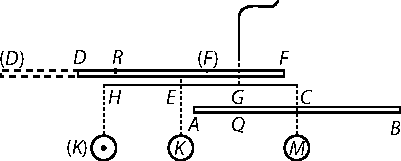
\includegraphics[scale=1]{gesamttex/edit_VIII-4/images/LH_35_09_10_001-002_d5_002v.pdf} 
\edcaption{\edtext{\lbrack\textit{Fig.~5}\rbrack}{%
\lemma{\lbrack\textit{Fig.~5}\rbrack}%
\Cfootnote[nonum]{Ein gestrichener Entwurf zum Diagramm wird nicht wiedergegeben. Leibniz zeichnet in \lbrack\textit{Fig.~5}\rbrack\ \textit{R} und \textit{D} als separate Punkte. Allerdings gilt gemäß den Angaben im Text $AB = CD$ sowie $QB = QR$ bzw. $= GR$. Daher müssen die Punkte \textit{R} und \textit{D} zusammenfallen. Der Fehler wirkt sich nicht auf die Argumentation aus.}}}
\end{edfigure}
\pstart
Soit la 
\edtext{balance\indexS{balance} \textit{CGEH}}{\lemma{balance}\Bfootnote{%
\textit{(1)}~\textit{EC} soutenue %
\textit{(2)}~\textit{CGEH}~\textit{L}}}
soutenue 
\edtext{en \textit{G}. Les bras \textit{GC} et \textit{GE} égaux, et deux corps egaux \textit{M}, \textit{K}}{\lemma{en \textit{G}.}\Bfootnote{%
\textit{(1)}~\textit{GC} et \textit{GE} égales, %
\textit{(2)}~Les bras \textit{GC} et \textit{GE} égaux,
\textit{(a)}~dont son %
\textit{(b)}~deux
\textit{(aa)}~\textit{M}, \textit{K} %
\textit{(bb)}~egaux \textit{M}, \textit{K}~\textit{L}}}
suspendus de ces bras,\indexS{bras de la balance} qui sont en equilibre.\indexS{equilibre} 
Changeons ces deux corps en deux parallelepipedes prismes ou cylindres egaux et egalement épais \textit{K} en \textit{DF} et \textit{M} en \textit{AB} 
\edtext{attachés 
\edlabel{35_09_10_001-002_7a}%
\edtext{}{%
\xxref{35_09_10_001-002_7a}{35_09_10_001-002_7b}%
\lemma{\textls{fermement} \lbrack...\rbrack\ \textls{fermement}}%
\Cfootnote{Das Wort ist in beiden Fällen doppelt unterstrichen.}}%
\textls{fermement} le long de la balance\bracks{,}}{\lemma{}\Bfootnote{attachés \textls{fermement} %
\textit{(1)}~à %
\textit{(2)}~le long de la balance \textit{erg.~L}}} 
soutenus en leur points de milieu\indexS{point de milieu} par 
\edtext{\bracks{\textit{C}}}{\lemma{}\Bfootnote{\textit{E} \textit{L ändert Hrsg.}}}
et \textit{F}. Il est manifeste que tout demeure en equilibre.\indexS{equilibre} Mais 
\edtext{avançons \textit{K} en (\textit{K}). Il est manifeste que c'est comme si nous avancions \textit{FD} en (\textit{F})(\textit{D}) et l'attachions \textls{fermement}\edlabel{35_09_10_001-002_7b} en \textit{H}. Prenons \textit{GR} égale à \textit{QB}. Il est manifeste que $QA+AR$ contrebalancent \textit{QB}. 
Or il y a encor \bracks{(\textit{F})}\textit{A}
et \textit{R}(\textit{D}) qui pesent du costé de \textit{GE} donc ce costé l'emporte.}{\lemma{avançons}\Bfootnote{%
\textit{(1)}~\textit{FD} en (\textit{F})(\textit{D}) %
\textit{(2)}~\textit{K} en (\textit{K}) \bars{en sorte \textit{erg.~u.~gestr.}}. Il est \bracks{...} en (\textit{F})(\textit{D})  
\textit{(a)}~par
\textit{(b)}~.~Or
\textit{(c)}~.~Alors
\textit{(d)}~.~Il est manifeste qu'il y a plus de poids alors du costé de \textit{GE} que du costé de \textit{GC}. Car du costé de \textit{GC} il n'y a que \textit{QB}; mais du costé de \textit{GE} il y a maintenant (\textit{F})(\textit{D})
\textit{(aa)}~egale à
\textit{(bb)}~et encor \textit{QA}. Et tout cela fait bien plus que \textit{QB}. Or lors qu'il y a plus de po
\textit{(e)}~et \lbrack...\rbrack\ que %
\textit{(aa)}~$QA+(F)R$  %
\textit{(aaa)}~contre %
\textit{(bbb)}~du costé de \textit{GE} %
\textit{(bb)}~$QA+AR$ \bracks{...} encor \bars{\textit{FA} \textit{ändert Hrsg.}} et \textit{R}(\textit{D})
 \bracks{...} l'emporte.~\textit{L}}}
\pend
\pstart \textls{Problème}: deux 
\edtext{corps estant}{%
\lemma{corps}\Bfootnote{%
\textit{(1)}~estan
\textit{(2)}~ine
\textit{(3)}~estant donnés 
\textit{(a)}~trouver leur
\textit{(b)}~la pr
\textit{(4)}~estant donnés, \bars{et \textit{streicht Hrsg.}}
\textit{(a)}~la place de l'un de deux dans la balance, trouver \bars{la place de \textit{streicht Hrsg.}} l'autre \bars{pour les mettre en equilibre. \textit{streicht Hrsg.}}
\textit{(b)}~trouver %
\textit{(aa)}~leur places %
\textit{(bb)}~leur places
\textit{(5)}~estant~\textit{L}}}
donnés, et leur Points dans la balance\bracks{,} trouver le point de l'equilibre\indexS{point de l'equilibre} ou du 
\edlabel{35_09_10_001-002_5a}%
\edtext{}{\xxref{35_09_10_001-002_5a}{35_09_10_001-002_5b}\lemma{soutien.}\Bfootnote{%
\textit{(1)}~Soyent les corps donnés
\textit{(a)}~\textit{ACB} 
\textit{(b)}~\bars{en forme de prismes egalement epais representés par les droites \textit{erg.}}
\textit{DEF} \textit{ACB} \bars{qui ont la meme raison entre elles que les corps \textit{erg.}}
\textit{(aa)}~et place de celuycy donnée, on cherche la place de l'autre. 
\textit{(aaa)}~Si (\textit{D})(\textit{E})(\textit{F}) estoit la veritable, il faudroit que 
\textit{(aaaa)}~$DG+$
\textit{(bbbb)}~$(A)G+$ 
\textit{(cccc)}~$AG+DG$ fût egale à
\textit{(bbb)}~Si (\textit{A})(\textit{C})(\textit{B}) et
\textit{(ccc)}~Si $AG+(D)G$ estoit égal à $GB+G(F)$
\textit{(ddd)}~Si $AG+DG$ estoit égal à $GB+GF$ tout s
\textit{(bb)}~on cherche leur places, c'est à dire
\textit{(aaa)}~les points
\textit{(bbb)}~celles des points de milieu \textit{C}, \textit{E}. Si \textit{AG} estoit égal à \textit{GF} et \textit{DG} à \textit{GB}, tout seroit en equilibre. Or si \textit{AG} egal à \textit{GF} donc $AC+CG$ égal à $GE+EF$. Et si \textit{DG} égal à \textit{GB} donc $DE-EG$ égal à $CB-CG$. Mais en ce cas \textit{AB} seroit égal à \textit{DF}
\textit{(2)}~\lbrack/\rbrack\ Soyent les corps donnés 
\textit{(a)}~\textit{DEF}, \textit{ACB}.
\textit{(b)}~en forme~\textit{L}}}%
soutien.
\pend 
\begin{edfigure}[0.5em][1em] 		%
\includegraphics[scale=1]{%
gesamttex/edit_VIII-4/images/LH_35_09_10_001-002_d6_002v.pdf}
\edcaption{\edtext{\lbrack\textit{Fig.~6}\rbrack}{%
\lemma{\lbrack\textit{Fig.~6}\rbrack}%
\Cfootnote[nonum]{Ein gestrichener Entwurf zum Diagramm wird nicht wiedergegeben. Auf die darin enthaltenen Punktebezeichnungen (\textit{A}), ... (\textit{F}) \textendash\ beziehen sich die gestrichenen Varianten \textit{(aaa)}\textendash\textit{(ccc)} zu \refpassage{35_09_10_001-002_5a}{35_09_10_001-002_5b}.}}}
\end{edfigure}
\pstart 
Soyent les corps donnés en forme\edlabel{35_09_10_001-002_5b} 
de prismes ayant l'epaisseur 
\edtext{égale, et les longueurs quelconques (selon que les prismes sont plus ou moins épais) \textit{DF},}{%
\lemma{égale,}%
\Bfootnote{%
\textit{(1)}~et representés
\textit{(2)}~et
\textit{(a)}~la longeur de ces droites
\textit{(b)}~les longueurs
\bars{quelconques \lbrack...\rbrack\ épais) \textit{erg.}}
\textit{DF},~\textit{L}}}
\textit{AB}, en raison\indexS{raison de deux corps} des 
\edtext{corps attachés}{\lemma{corps}\Bfootnote{%
\textit{(1)}~ou des %
\textit{(2)}~suspendus
\textit{(3)}~attachés à la balance %
\textit{(3)}~en \textit{E}, \textit{C}. Leur points de milieu et extremites de la dite balance %
\textit{(4)}~attachés~\textit{L}}}
le long de la balance en sorte que \textit{E}, \textit{C} leur points de milieu\indexS{point de milieu} sont 
\edtext{l\lbrack es\rbrack}{\lemma{}\Bfootnote{l' \textit{L ändert Hrsg.}}}
extremités de la dite balance.
On demande le point de milieu\indexS{point de milieu} \textit{G}. %
\pend
\pstart
Soit \textit{BXZ} egale à \textit{DEF} et leurs points de milieu, \textit{X}, \textit{E} egalement distans de \textit{G}, c'est à dire \textit{XG} égale 
\edtext{à \textit{EG}. Enfin}{\lemma{à \textit{EG}.}\Bfootnote{%
\textit{(1)}~De plus \textit{A} %
\textit{(2)}~Enfin $FA+AG$ égal à \textit{ZG}. %
\textit{(3)}~Enfin~\textit{L}}}
\textit{FG} ou \textit{AG} (posant qu'\textit{AB} commence où \textit{DF} finit) egal à \textit{ZG}.
\edtext{Ainsi \textit{DF}}{\lemma{Ainsi}\Bfootnote{%
\textit{(1)}~\textit{BZ} sera %
\textit{(2)}~\textit{DF}~\textit{L}}}
sera contrabalancée par \textit{BZ} et \textit{AZ} 
\edtext{ou \textit{FZ} de soy même. Donc}{\lemma{ou \textit{FZ}}\Bfootnote{%
\textit{(1)}~par luy même %
\textit{(2)}~de soy même. %
\textit{(a)}~Donc \textit{BC} egal à \textit{GE} %
\textit{(b)}~Donc~\textit{L}}}
\textit{G} est au 
\edtext{milieu. Or}{\lemma{milieu.}\Bfootnote{%
\textit{(1)}~De plus \textit{AG} estant \textit{FG}, donc \textit{EG} égale 
\textit{(a)}~\textit{AC}
\textit{(b)}~à \textit{AC}
\textit{(c)}~\bars{à \textit{AC} \textit{streicht Hrsg.}}
\textit{(2)}~Or~\textit{L}}}
puisque \textit{GZ} egale à \textit{GA}, donc 
\edtext{$BG-DF$ egale}{\lemma{$BG-DF$}\Bfootnote{%
\textit{(1)}~c'est à dire %
\textit{(2)}~egale~\textit{L}}}
à \textit{GA}. C'est à dire $BC+CG-DF$ egale à $AC-CG$. Et \textit{AC} estant egale à \textit{BC} nous aurons $2\,CG$ egale à \textit{DF}. C'est à dire \textit{CG} egale à \textit{FE} ou \textit{DE}, donc \textit{CA} (ou $CG+GA$) egale à \textit{GE} (ou 
\edtext{$GA+FE$). Donc \textit{CG} à}{\lemma{$GA+FE$).}\Bfootnote{%
\textit{(1)}~C'est à dire %
\textit{(2)}~Donc \textit{CG}
\textit{(a)}~égale %
\textit{(b)}~à~\textit{L}}}
\textit{GE} comme \textit{DF} à \textit{AB}, c'est à dire les bras 
\edtext{dont les corps sont suspendus en equilibre,\indexS{corps suspendus en equilibre}\indexS{equilibre} sont}{\lemma{}\Bfootnote{dont les corps
\bars{qu'en \textit{erg.~u.~gestr.}} sont suspendus en equilibre, sont \textit{erg.~L}}} 
en raison reciproque\indexS{raison reciproque de deux corps} des 
\edtext{corps. Ainsi nous rencontrons enfin la regle}{\lemma{corps.}\Bfootnote{%
\textit{(1)}~Et nous avons la solution du probleme conforme au theoreme %
\textit{(2)}~Ainsi nous rencontrons enfin %
\textit{(a)}~le theoreme co %
\textit{(b)}~la regle~\textit{L}}}
vulgaire de l'equilibre,\indexS{regle vulgaire de l'equilibre} par une espece 
\edtext{d'Analyse\indexS{Analyse} et}{\lemma{d'Analyse}\Bfootnote{%
\textit{(1)}~et sans l'avoir sçeue. %
\textit{(2)}~et~\textit{L}}}
comme si nous en avions rien sçeu.
\pend
\pstart 
\edtext{La chose}{\lemma{}\Bfootnote{La  \bars{seule \textit{gestr.}} chose~\textit{L}}}
qui reste à mon 
\edtext{avis, pour}{\lemma{}\Bfootnote{%
avis, \bars{à faire \textit{gestr.}}  pour perfectionner~\textit{L}}}
perfectionner cette meditation, c'est 
\foreignlanguage{ngerman}{\lbrack\textit{Text bricht~ab.}\rbrack}
\pend
\selectlanguage{ngerman}
